%==============================================================================
%  Isolating the Determinants of Human-Like Motion in Reinforcement Learning
%  Control of a 2-DOF Robotic Arm
%
%  Ranjot Singh Sandhu, Wilfrid Laurier University
%==============================================================================
\documentclass[conference]{IEEEtran}
\IEEEoverridecommandlockouts

\usepackage{cite}
\usepackage{amsmath,amssymb,amsfonts}
\usepackage{graphicx}
\usepackage{textcomp}
\usepackage{booktabs}
\usepackage{url}
% Keeps floats from drifting past the section they belong to, and in
% particular stops any figure or table landing after the references.
\usepackage{placeins}

\begin{document}

\title{Isolating the Determinants of Human-Like Motion in\\
Reinforcement Learning Control of a 2-DOF Robotic Arm}

\author{\IEEEauthorblockN{Ranjot Singh Sandhu}
\IEEEauthorblockA{\textit{Department of Physics and Computer Science} \\
\textit{Wilfrid Laurier University}\\
Waterloo, Canada \\
sand0301@mylaurier.ca}
}

\maketitle

%==============================================================================
\begin{abstract}
Robot arms trained with reinforcement learning reach their targets, but they
usually do not move the way people move. Fischer et al. (2021) showed that a
soft actor-critic (SAC) agent trained on a simulated human arm with muscles
reproduced two well-known laws of human movement: Fitts' Law and the two-thirds
power law. Their setup changed many things at once, so it could not show which
part caused the effect. We rebuilt their method on a small 2-DOF planar arm
that trains in about half an hour, which made controlled tests affordable. We
report two results. First, muscle actuation did not help. When we gave both
actuation types the same 500{,}000-step budget and used the same random seeds
in each condition, muscle actuation gave power-law exponents that were
\emph{further} from the biological value of $-1/3$ than simple joint-velocity
control ($-0.445 \pm 0.108$ against $-0.343 \pm 0.083$; paired $t$-test,
$p=0.038$). Neither condition was statistically different from $-1/3$ on its
own. An earlier version of this comparison seemed to show the opposite, but
only because the velocity baseline had been trained for one fifth as long.
Second, on a harder three-waypoint task, agents learned to travel between
targets but not to stop and hold at the last one. Testing four possible fixes
showed that saving the best checkpoint during training was the one that
mattered: the saved checkpoint solved the task in 20 out of 20 trials, while
the final model from the same training run solved it 0 out of 20.
\end{abstract}

\begin{IEEEkeywords}
reinforcement learning, soft actor-critic, muscle model, motor control,
Fitts' Law, two-thirds power law, curriculum learning, robotic arm
\end{IEEEkeywords}

%==============================================================================
\section{Introduction}

Reinforcement learning (RL) controllers for robot arms are normally judged on
whether they reach the target and how fast. By that measure they work well. But
the paths they produce are often jerky and unnatural. This matters for
prosthetic limbs, rehabilitation devices, and robots that work next to people,
where moving in a human-like way is part of the job.

Human arm movement follows two well-tested rules. Fitts' Law \cite{fitts1954}
says that the time $MT$ to reach a target grows with how hard the target is to
hit:
\begin{equation}
MT = a + b \cdot \mathrm{ID}, \qquad
\mathrm{ID} = \log_2\!\left(\frac{2D}{W}\right),
\label{eq:fitts}
\end{equation}
where $D$ is the distance to the target and $W$ is its width. The two-thirds
power law \cite{lacquaniti1983} says that the hand slows down on tight curves:
\begin{equation}
V \propto C^{-1/3},
\label{eq:power}
\end{equation}
where $V$ is speed and $C$ is curvature. Fitting $\log V$ against $\log C$
should give a slope near $-0.333$. Together these give a clear numerical test
of whether a robot moves like a person.

Fischer et al. \cite{fischer2021} trained a SAC agent on a 7-DOF model of the
human arm in MuJoCo \cite{todorov2012}, driven by simulated muscles. The
trained agent reproduced both laws. Their system, however, combined a detailed
muscle model, a curriculum, a shaped reward, and a specific RL algorithm. From
that work alone we cannot tell which ingredient produced the human-like motion.

This paper tests that question directly. We rebuilt the method on a 2-DOF
planar arm. The arm is small enough to train fully in about thirty minutes on
an ordinary desktop CPU, so we could run the same experiment many times and
change one thing at a time. Our questions were:

\begin{itemize}
\item[\textbf{RQ1.}] Does a SAC agent on a 2-DOF arm reproduce Fitts' Law and
the two-thirds power law?
\item[\textbf{RQ2.}] With everything else held fixed, does muscle actuation
explain the human-like motion?
\item[\textbf{RQ3.}] Does the method extend to visiting several waypoints in
order and holding position at the end?
\end{itemize}

Our contributions are: a working open implementation that runs on ordinary
hardware; a matched, seed-paired test showing that muscle actuation does
\emph{not} improve the power-law match, plus a demonstration of how easily an
unmatched training budget gives the opposite answer; and an ablation on the
waypoint task showing that keeping the best checkpoint during training is what
decides success.

%==============================================================================
\section{Background}
\label{sec:background}

\subsection{RL for muscle-driven control}

Soft actor-critic \cite{haarnoja2018} is an off-policy algorithm that adds an
entropy bonus to encourage exploration. It is more sample-efficient than
on-policy methods such as PPO \cite{schulman2017}, which is why we use it here.

Controlling muscles is harder than controlling torques. A muscle can only pull,
never push, so each joint needs two of them working against each other. This
doubles the size of the action space and lets the agent waste effort by pulling
both ways at once. Larger benchmarks for this kind of control exist, including
MyoSuite \cite{caggiano2022} and the ``Learn to Move'' competitions
\cite{kidzinski2020}. Our 2-DOF arm is far smaller than those and is not meant
to compete with them. Its value is that it is cheap enough to run controlled
comparisons many times over.

\subsection{Two explanations for human movement laws}

There are two main explanations for why human movement follows these laws, and
they predict different things about our experiment.

The first says the laws come from \emph{planning}. The minimum-jerk model of
Flash and Hogan \cite{flash1985} shows that paths which minimise jerk match
real human reaching, and the two-thirds power law falls out of that smoothness
as a side effect. Optimal feedback control \cite{todorov2002} makes a similar
argument from cost minimisation. If this view is right, an agent trained to
reach smoothly should show the power law \emph{whatever} actuator it uses.

The second says the laws come from the \emph{body}. On this view the muscles
themselves, and in particular the fact that a muscle gets weaker the faster it
shortens, force the speed-curvature relationship without anything having to
plan it. If this view is right, changing the actuator should change the
exponent.

Viviani and Flash \cite{viviani1995} review the disagreement, which is still
open. Our experiment in Section~\ref{sec:results} can tell the two apart.

\subsection{Muscle model and curriculum}

The Hill muscle model \cite{hill1938} writes muscle force as activation times a
force-length term times a force-velocity term. The force-velocity term is the
important one here: it weakens the muscle as it shortens faster, which puts a
speed penalty into the physics rather than into the reward.

Curriculum learning \cite{bengio2009} trains on easy cases first. Fischer et
al.\ applied this to the goal size, starting with a wide target and shrinking
it as the agent improved, because a small target gives almost no learning
signal at the start. Our reward shaping follows the potential-based form of Ng
et al.\ \cite{ng1999}, which speeds up learning without changing the best
policy.

%==============================================================================
\section{Method}

\subsection{The arm and the environment}

The arm has two links in a plane, as shown in Fig.~\ref{fig:system}(a). We
built it as a Gymnasium \cite{towers2024} environment and trained it with
Stable-Baselines3 \cite{raffin2021}. Parameters are in
Table~\ref{tab:params}. Each episode starts with the arm hanging straight down
and ends after at most 1000 steps. Note that the elbow is already limited to
the human range of $0$--$120^{\circ}$; the shoulder is not limited.

\begin{figure*}[t]
\centerline{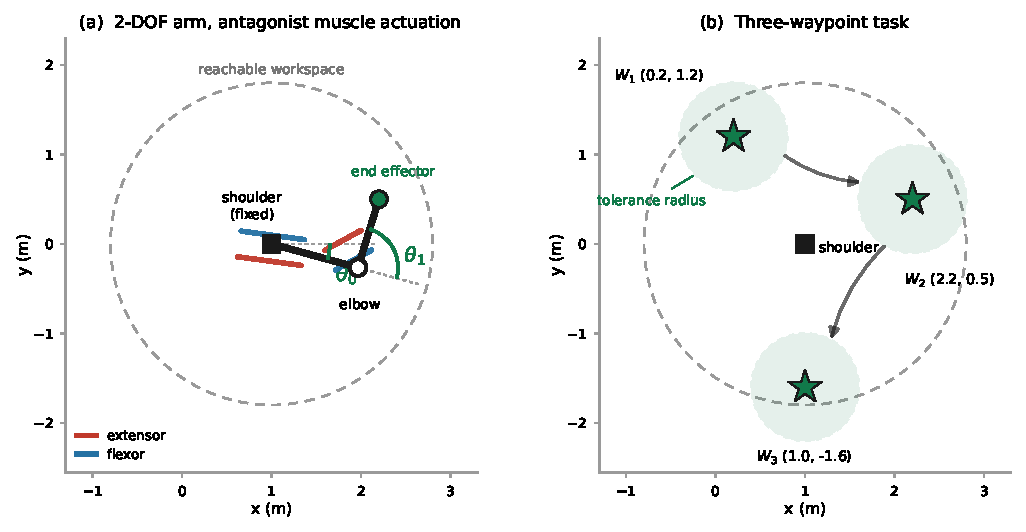
\includegraphics[width=\textwidth]{figures/system.pdf}}
\caption{(a) The 2-DOF arm. The shoulder is fixed and the two links give a
1.80~m reach. In muscle mode each joint is driven by a pair of Hill-type
muscles pulling against each other, so the agent outputs four muscle
activations instead of two joint velocities. (b) The three-waypoint task. The
arm must visit $W_1$, $W_2$, $W_3$ in order. Shaded circles show the 0.60~m
tolerance. The first two waypoints only need to be touched; the last one must
be held for 20 steps in a row.}
\label{fig:system}
\end{figure*}

The agent sees an 11-number observation:
\begin{equation}
\begin{split}
\mathbf{o} = \big[&\sin\theta_0,\ \cos\theta_0,\ \sin\theta_1,\ \cos\theta_1,\\
&\hat{\omega}_0,\ \hat{\omega}_1,\ e_{\parallel},\ \phi,\ \hat{g},\
\mathbb{1}_{\text{goal}},\ h/H \big].
\end{split}
\label{eq:obs}
\end{equation}
Joint angles are given as sine and cosine so there is no jump at $\pm\pi$.
$\hat{\omega}_j$ are joint speeds scaled to $[-1,1]$. $e_{\parallel}$ is the
position error along the direction of the goal, $\phi$ the orientation error,
and $\hat{g}$ a scaled measure of how fast the error is changing.
$\mathbb{1}_{\text{goal}}$ is 1 when the arm is inside the goal region. $h/H$
is how much of the required hold has been completed. The last two let the agent
tell the difference between approaching a target and holding at it.

\begin{table}[htbp]
\caption{Arm and Muscle Parameters}
\begin{center}
\setlength{\tabcolsep}{4pt}
\begin{tabular}{llc}
\toprule
\textbf{Parameter} & \textbf{Symbol} & \textbf{Value} \\
\midrule
Shoulder position & --- & $[1.0,\ 0.0]$ m \\
Link lengths & $\ell_0, \ell_1$ & $1.00,\ 0.80$ m \\
Maximum reach & --- & $1.80$ m \\
Link masses & $m_0, m_1$ & $2.0,\ 1.5$ kg \\
Joint inertias & $I_0, I_1$ & $0.10,\ 0.08$ kg\,m$^2$ \\
Joint damping & $b$ & $0.10$ N\,m\,s/rad \\
Shoulder range & $\theta_0$ & $[-\pi,\ \pi]$ rad \\
Elbow range & $\theta_1$ & $0$--$120^{\circ}$ \\
Speed limit & $\omega_{\max}$ & $2.0$ rad/s \\
Time step & $\Delta t$ & $0.01$ s \\
\midrule
Max muscle force & $F_{\max}$ & $100$ N \\
Optimal fibre length & $L_{\mathrm{opt}}$ & $0.10$ m \\
Max shortening speed & $v_{\max}$ & $10\ L_{\mathrm{opt}}$/s \\
Force-length width & $\sigma_L$ & $0.45$ \\
Eccentric plateau & $F_{\mathrm{ecc}}$ & $1.5\,F_{\max}$ \\
Moment arm & $r$ & $0.05$ m \\
\bottomrule
\end{tabular}
\label{tab:params}
\end{center}
\end{table}

\subsection{The two actuation modes}
\label{sec:actuation}

The actuation mode is the thing we change. Both modes sit behind the same
interface, so the environment, reward, and training code are shared.

\textbf{Velocity mode (baseline).} The action is two numbers in $[-1,1]$, read
as joint speed commands and applied directly:
\begin{equation}
\theta_{t+1} = \theta_t + a \cdot \omega_{\max} \cdot \Delta t .
\label{eq:velocity}
\end{equation}
There is no force or inertia in this mode; the commanded speed happens
immediately.

\textbf{Muscle mode.} The action is four numbers in $[0,1]$: one extensor and
one flexor per joint. Each muscle produces force
\begin{equation}
F = a \cdot F_{\max} \cdot f_L(\hat{L}) \cdot f_V(\hat{v}),
\label{eq:hill}
\end{equation}
with normalised length $\hat{L}$ and speed $\hat{v}$. The force-length curve is
the Gaussian form of Thelen \cite{thelen2003},
\begin{equation}
f_L(\hat{L}) = \exp\!\left[-\left(\frac{\hat{L}-1}{\sigma_L}\right)^{\!2}\right],
\label{eq:fl}
\end{equation}
which matches the curves reported by Zajac \cite{zajac1989}. The
force-velocity curve is
\begin{equation}
f_V(\hat{v}) =
\begin{cases}
\max(0,\ 1 - \hat{v}), & \hat{v} \geq 0,\\[3pt]
F_{\mathrm{ecc}} - (F_{\mathrm{ecc}}-1)\,e^{k\hat{v}}, & \hat{v} < 0,
\end{cases}
\label{eq:fv}
\end{equation}
with $k = 1/(F_{\mathrm{ecc}}-1)$. Both branches give $f_V(0)=1$ and have
matching slopes at zero.

One point is worth stating plainly: the shortening branch of (\ref{eq:fv}) is a
straight line, not the curved Hill hyperbola. It keeps the two properties that
matter here, namely that force drops as shortening speed rises and reaches zero
at $v_{\max}$, but its exact shape is not the textbook one. A curved version
might behave differently.

The two muscles at a joint produce a net torque through the moment arm $r$,
which is integrated against the joint inertia with damping:
\begin{equation}
\tau = r\,(F_{\mathrm{ext}} - F_{\mathrm{flex}}) - b\,\omega, \qquad
\alpha = \frac{\tau}{I}.
\label{eq:torque}
\end{equation}
Muscle mode adds no reward term. Any difference in the motion comes from the
physics in (\ref{eq:hill})--(\ref{eq:torque}).

\subsection{Reward}

The reward has six penalties that apply every step, three bonuses that apply
under certain conditions, and a bonus at the end:
\begin{equation}
\begin{split}
R = &-2.0\,d - 1.0\,\phi - 0.15\lVert \omega \rVert
     - 0.20\,\hat{g} \\ &- 0.01\lVert a \rVert - 0.08\,\kappa
     + B_{\text{prog}} + B_{\text{prox}} + B_{\text{hold}},
\end{split}
\label{eq:reward}
\end{equation}
where $d$ is distance to the goal, $\phi$ the orientation error,
$\lVert\omega\rVert$ the joint speed, $\hat{g}$ the error-change term,
$\lVert a\rVert$ the size of the action, and $\kappa$ the average
co-contraction (always zero in velocity mode, which has no muscle pairs).

The bonuses are: $B_{\text{prog}} = 1.5\Delta$ when the total error $E = 2d +
\phi$ drops by $\Delta$; $B_{\text{prox}} = 4.0\,(1 - d/3\rho)$ when the arm is
within three times the goal radius $\rho$; and $B_{\text{hold}} = 10 + 2h$
while the arm is inside the goal region, where $h$ is the hold counter. A bonus
of $+150$ is given once on success, and $+25$ each time an intermediate
waypoint is reached.

The same reward and the same weights are used in both actuation modes. Two of
the ten terms cannot be exactly equal, because they depend on the action and
the action spaces differ: $\lVert a \rVert$ is computed over two numbers in
velocity mode and four in muscle mode, and $\kappa$ is always zero in velocity
mode. Their weights, $0.01$ and $0.08$, are the two smallest in the reward and
are far below the distance penalty ($2.0$), the in-goal bonus ($10$), and the
success bonus ($150$), so their effect is small.

\subsection{Goal region, hold, and curriculum}
\label{sec:curriculum}

The arm is \emph{in the goal region} when all three of
\begin{equation}
d < \rho, \qquad \phi < 12^{\circ}, \qquad
\lVert \omega \rVert < 0.3\ \mathrm{rad/s}
\label{eq:ingoal}
\end{equation}
hold at the same time. The hold counter then changes as
\begin{equation}
h_{t+1} =
\begin{cases}
h_t + 1, & \text{in the goal region},\\
\max(0,\ h_t - \delta), & \text{otherwise},
\end{cases}
\label{eq:hold}
\end{equation}
and the episode succeeds when $h \geq H$. We use a partial decrease rather than
resetting to zero, because a reset makes one bad step wipe out all progress. We
lowered $\delta$ from 5 to 3 during development on the assumption that a gentler
penalty would help. Section~\ref{sec:ablation} tests that assumption and does
not support it, so we treat $\delta$ as an open choice.

Two curricula run during training. The \emph{tolerance curriculum} starts the
goal radius at $0.60$~m and multiplies it by $0.80$ once four conditions hold: a
50-episode window is full, at least 20 episodes have passed since the last
change, the radius is above its floor, and the success rate is at least 80\%.
The floor is $0.02$~m for single targets and $0.20$~m for the waypoint task.
The \emph{hold curriculum} raises $H$ through $\{10,15,20\}$ once the success
rate reaches 60\%.

We found and fixed two faults in our first version. The success window was not
cleared when a stage changed, so old easy episodes could trigger a second
change straight away and make the task suddenly much harder. We now clear it.
Also, success was measured from the exploring policy, whose noise breaks the
hold and makes the agent look worse than it is. Both curricula are now driven
by separate deterministic tests, and only one difficulty increase is allowed
per test.

\subsection{Tasks}
\label{sec:tasks}

\textbf{Single target.} The arm reaches a fixed direction and holds inside the
tolerances of (\ref{eq:ingoal}) for 20 steps. This is the task used for the
Fitts' Law and power-law tests.

\textbf{Three waypoints.} The arm visits $W_1 = [0.2, 1.2]$, $W_2 = [2.2,
0.5]$, and $W_3 = [1.0, -1.6]$ in order (Fig.~\ref{fig:system}(b)). These sit
$1.30$--$1.60$~m from the shoulder, well inside the $1.80$~m reach, and
$2.1$--$2.9$~m apart. The first two only need the distance condition; the last
needs the full condition and the complete hold.

\subsection{Training setup}

Every run uses SAC with an MLP policy of two 256-unit layers, learning rate
$3\times10^{-4}$, replay buffer of $200{,}000$, batch size $256$, and
$500{,}000$ training steps. Early tests showed little gain past $500$K.

Because results vary a lot between random seeds, we train seeds in parallel and
seed Python, NumPy, and PyTorch explicitly so runs can be repeated exactly. On
the waypoint task we also test the policy every $25{,}000$ steps on five
deterministic episodes and save the best-scoring model separately from the
final one.

Two automatic tests measure the movement laws. The Fitts' Law test sweeps six
distances ($0.20$ to $1.20$~m) against six widths ($0.02$ to $0.30$~m), giving
36 conditions, and runs 10 trials each with a 200-step cap. Conditions where no
trial succeeded are left out of the fit. The power-law test runs 20 reaching
trials, takes a speed and curvature reading at every step, drops readings below
$0.01$~m/s or $0.10$~m$^{-1}$ because both go into logarithms, and fits $\log
V$ against $\log C$.

The code is also covered by 50 unit tests over the environment, kinematics,
model wrappers, and plotting. At the time of writing 48 pass; the two failures
are a floating-point tolerance issue in a joint-limit check and an intermittent
plotting fault, neither of which touches training or evaluation.

%==============================================================================
\section{Results}
\label{sec:results}

\subsection{Actuation: a first comparison that was wrong}

Our first comparison used a velocity run trained for $100{,}000$ steps against
muscle runs at $200{,}000$ and $500{,}000$ steps. It looked convincing. The
velocity exponent was $-0.620$, almost double the biological value, while the
best muscle run reached $-0.330$, only $0.003$ away from $-1/3$. That is a
factor of 92 in error, and it appears to support the ``body'' explanation from
Section~\ref{sec:background}.

It was wrong. Training length was mixed up with actuation type. We report it
here because it was persuasive and false, which is the more useful lesson.

\subsection{Actuation: the matched comparison}

We retrained both modes at the same $500{,}000$ steps on the same task, using
the \emph{same random seeds} in each condition so that seed luck cannot explain
any difference. Table~\ref{tab:actuation} gives the result.

\begin{table}[htbp]
\caption{Matched Comparison, 500K Steps, Paired Seeds}
\begin{center}
\setlength{\tabcolsep}{5pt}
\begin{tabular}{lccc}
\toprule
\textbf{Seed} & \textbf{Velocity} & \textbf{Muscle} & \textbf{Difference} \\
\midrule
42  & $-0.3007$ & $-0.4196$ & $+0.1189$ \\
201 & $-0.4387$ & $-0.5634$ & $+0.1247$ \\
202 & $-0.2907$ & $-0.3518$ & $+0.0611$ \\
\midrule
mean $\pm$ sd & $-0.343 \pm 0.083$ & $-0.445 \pm 0.108$ & $+0.102$ \\
vs.\ $-1/3$ & $p = 0.85$ & $p = 0.22$ & --- \\
\bottomrule
\end{tabular}
\label{tab:actuation}
\end{center}
\end{table}

Three things follow.

\textbf{Muscle actuation did not help.} Its mean exponent of $-0.445$ is
further from $-1/3$ than the velocity mean of $-0.343$. The earlier conclusion
is reversed.

\textbf{The difference is consistent but small.} Velocity gave a less negative
exponent than muscle for all three matched seeds, by $0.06$ to $0.12$. A paired
$t$-test gives $t = 4.999$, $p = 0.038$, Cohen's $d = 1.06$. Pairing is the
right test because it cancels out seed-to-seed variation. Unpaired tests are
not significant (Welch $p = 0.27$, Mann-Whitney $p = 0.40$), which shows how
big the variation between seeds is compared with the effect.

\textbf{Neither mode differs from the biological value.} A one-sample test
against $-1/3$ does not reject for velocity ($p = 0.85$) or muscle ($p =
0.22$). Both actuators give a speed-curvature relationship consistent with the
human exponent. What differs is a small, steady offset, not whether the law
appears at all.

So RQ2 is answered no. Muscle actuation is not needed to get the power law,
because the law appears without it, and it does not improve the match. This
supports the planning explanation over the body explanation: an agent trained
to reach smoothly shows the pattern with either actuator, which is what
minimum-jerk and optimal-feedback accounts predict
\cite{flash1985,todorov2002}.

Fig.~\ref{fig:power} shows a typical speed-curvature plot. It is included to
show that the relationship is well formed, not as evidence for either mode,
since one run cannot serve that purpose given the variation above.

\begin{figure}[htbp]
\centerline{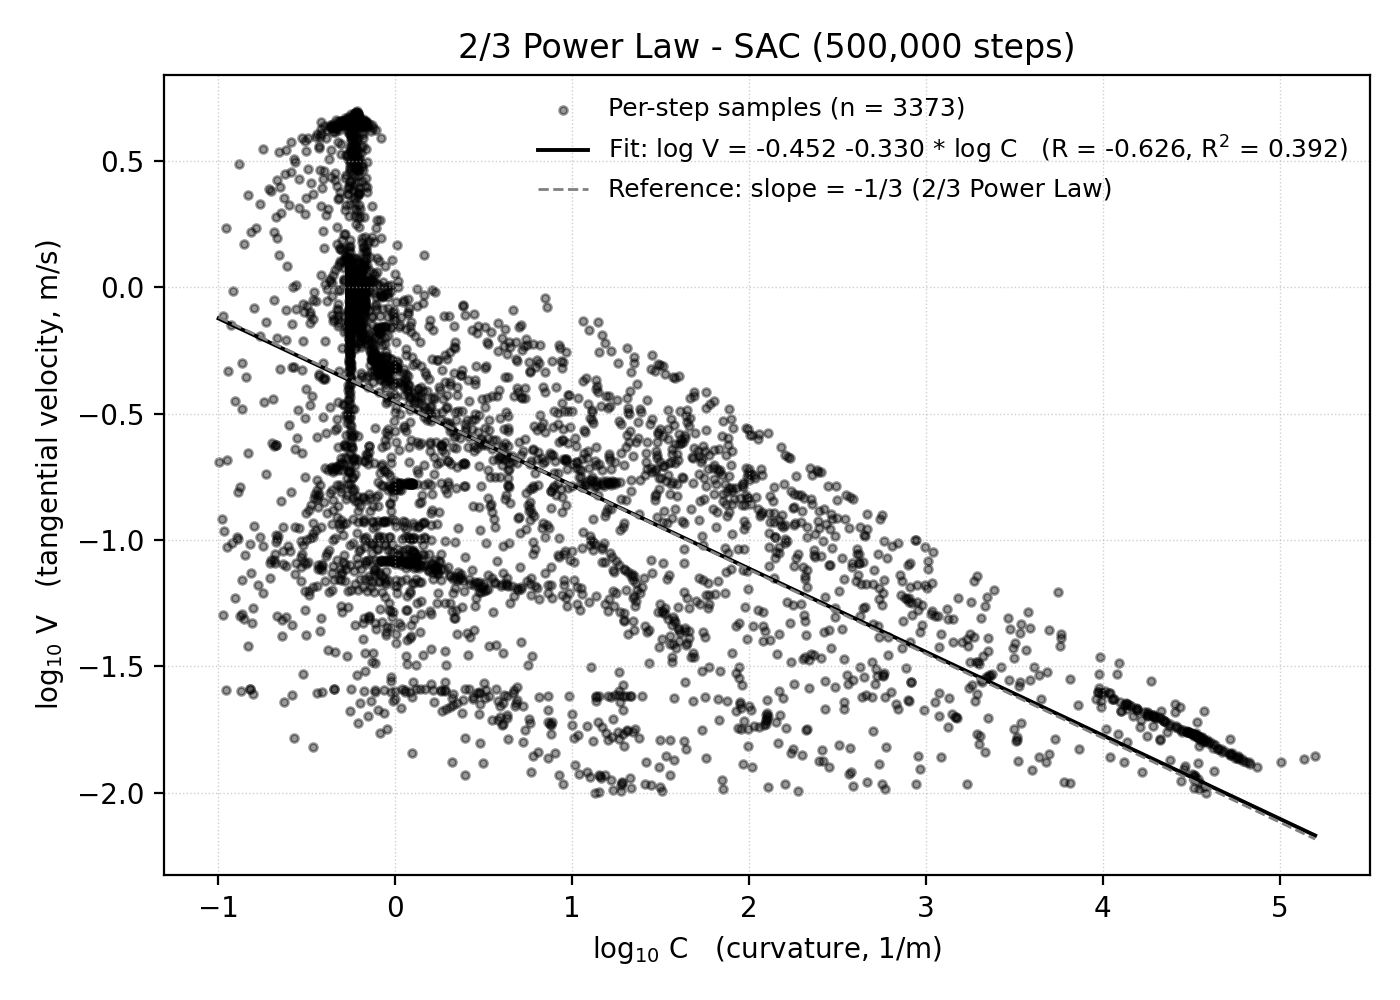
\includegraphics[width=0.92\columnwidth]{figures/power_law_muscle500k.png}}
\caption{A typical speed-curvature fit, here from a muscle-mode run. Each point
is one reading from a reaching trial. The band is clearly linear in log-log
coordinates, but the fitted exponent for any single run varies a lot with seed
(Table~\ref{tab:actuation}), so no one fit should be taken as representing its
condition.}
\label{fig:power}
\end{figure}

\textbf{Limits of this test.} Three matched pairs is a small sample. The paired
result at $p = 0.038$ is borderline and one more seed could push it either way.
The safe conclusions are the negative one, that muscle actuation gave no
advantage here, and the methodological one, that the unmatched comparison gave
the opposite answer and looked convincing doing it.

\subsection{Fitts' Law}

The Fitts' Law fit for a 500K muscle run gives $R^2 = 0.531$, with a slope of
$0.0364$~s/bit over 20 of the 36 conditions, plotted in Fig.~\ref{fig:fitts}.
That slope means about 27 bits per second, which is inside the human range.
Movement time rises steadily with difficulty, so the pattern is there, but the
fit is much weaker than Fischer's $R^2 = 0.999$.

\begin{figure}[!t]
\centerline{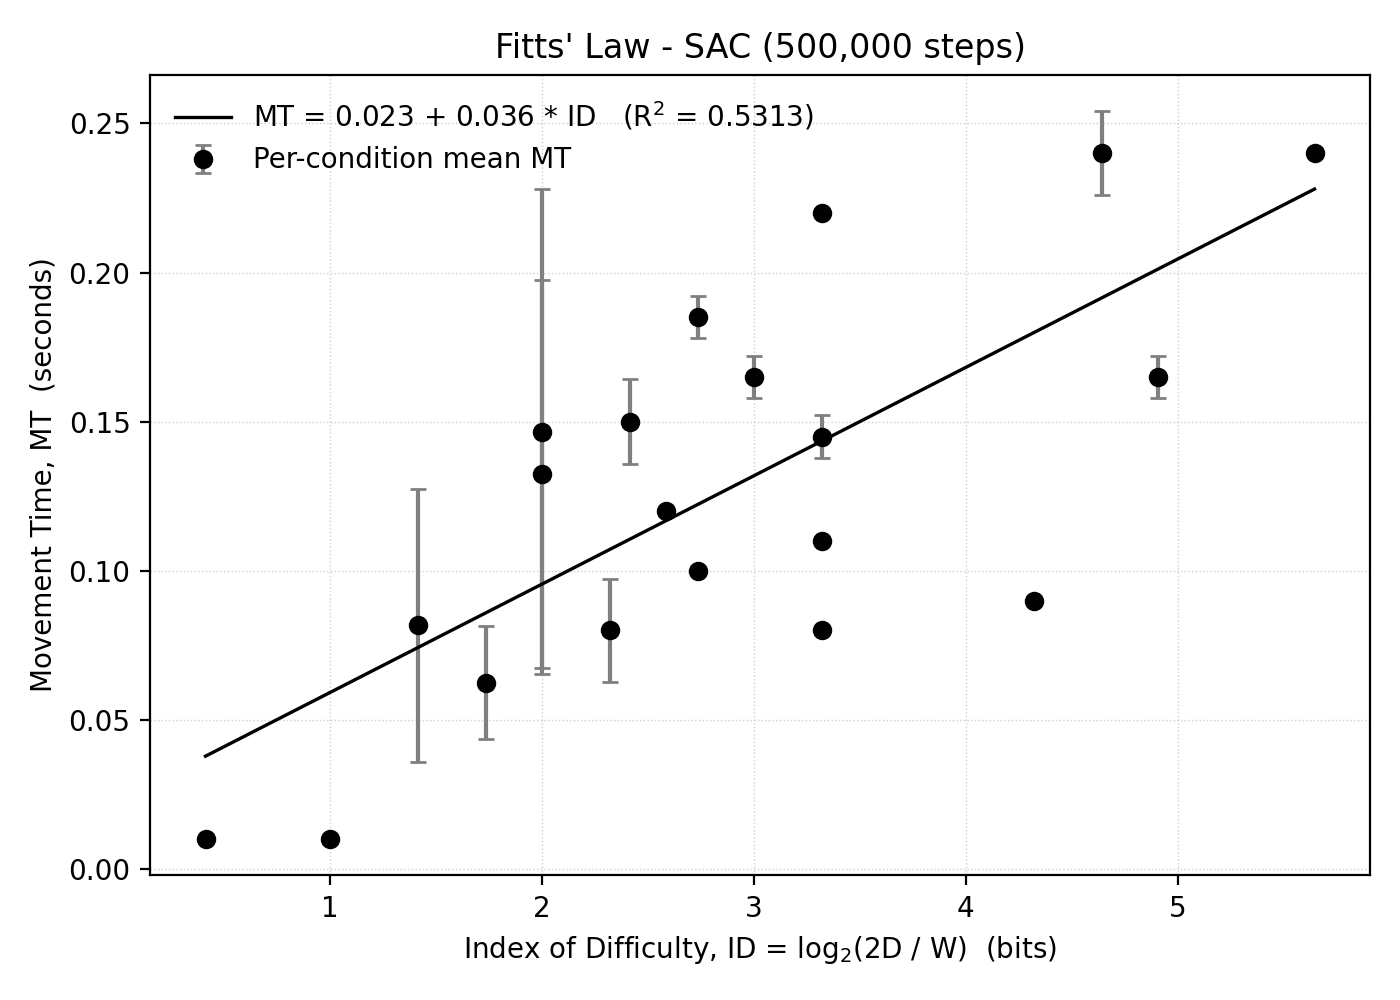
\includegraphics[width=0.92\columnwidth]{figures/fitts_law_muscle500k.png}}
\caption{Fitts' Law fit for a 500K muscle-mode run. Movement time rises
steadily with the index of difficulty, so the relationship holds, but the
spread at high difficulty is large. Those conditions use the smallest targets,
which the tolerance curriculum never reached during training.}
\label{fig:fitts}
\end{figure}

The reason is identifiable, and it is not simply too little training. The 500K
run advanced the tolerance curriculum \emph{once}, finishing at $0.480$~m,
while a 200K run advanced it \emph{twice}, reaching $0.384$~m, and scored
slightly better on Fitts' Law ($R^2 = 0.582$) with less than half the training.
Curriculum progress is therefore not guaranteed by training longer. The
curriculum advances on a rolling success rate, and an agent that settles into a
behaviour below the threshold can stay there no matter how many more steps it
gets. The smallest targets in the Fitts grid are never trained on, so those
conditions add scatter. This also explains why the two laws move in opposite
directions between runs: the power law is measured from the shape of free
movement and does not care where the curriculum stopped, while Fitts' Law
depends directly on final accuracy.

\subsection{Three waypoints: what goes wrong}

Thirty seeds completed the full budget on the waypoint task, using about
$10.8$ million environment steps and 70 hours of training in total.
Table~\ref{tab:seeds} summarises them.

\begin{table}[htbp]
\caption{Waypoint Seed Search (30 Completed Runs)}
\begin{center}
\setlength{\tabcolsep}{4pt}
\begin{tabular}{lc}
\toprule
\textbf{Measure} & \textbf{Value} \\
\midrule
Mean reward: min / median / max & $-7{,}007$ / $700$ / $31{,}565$ \\
Hold progress: min / median / max & $0.00$ / $0.00$ / $0.95$ \\
Runs with mean reward $> 25{,}000$ & $6 / 30$ \\
\textbf{Runs completing the full hold} & $\mathbf{0 / 30}$ \\
\bottomrule
\end{tabular}
\label{tab:seeds}
\end{center}
\end{table}

The last row is the key number. Six runs learned the task well enough to pass a
mean reward of $25{,}000$, and not one finished the hold at the final waypoint.
Agents reliably reached the first two waypoints and reached the third, but
could not stay there. The problem is not navigation, which is solved, but
stopping.

This makes sense given the actuator. Under velocity control, stopping is
trivial: command zero speed. Under muscle control there is no such command, and
the agent must balance two opposing muscles against leftover momentum.

\subsection{Testing four possible fixes}
\label{sec:ablation}

We proposed four fixes: a gentler hold penalty ($\delta = 3$ instead of 5); a
hold curriculum raising $H$ from 10 to 20; driving the curricula from
deterministic tests instead of the exploring policy; and keeping the best
checkpoint instead of the final model. Rather than assume these helped, we
turned each off in turn and measured. Each condition used three matched seeds
at the full budget. Checkpointing is measured inside every condition by scoring
both the saved checkpoint and the final model of the same run. Results are in
Table~\ref{tab:ablation}.

\begin{table}[htbp]
\caption{Ablation of the Four Fixes (3 Seeds Each)}
\begin{center}
\setlength{\tabcolsep}{4pt}
\begin{tabular}{lccc}
\toprule
\textbf{Condition} & \textbf{Mean wp.} & \textbf{Max hold} &
\textbf{Successes} \\
\midrule
All fixes on & $2.00$ & $0.02$ & $0/15$ \\
No hold curriculum & $1.00$ & $0.28$ & $0/15$ \\
$\delta = 5$ (not 3) & $1.67$ & $0.33$ & $\mathbf{5/15}$ \\
Old curriculum signal & $1.33$ & $0.38$ & $0/15$ \\
\bottomrule
\end{tabular}
\label{tab:ablation}
\end{center}
\end{table}

Two results stand out, and one of them goes against a choice we had already
made.

\textbf{Checkpointing decides the outcome.} The only successful policy came
from the $\delta = 5$ condition. Tested on 20 deterministic episodes at the
$0.6$~m standard with the full 20-step hold, its saved checkpoint succeeded
$20/20$, finishing in exactly 490 steps every time. The final model from the
\emph{same run}, under the same test, succeeded $0/20$: it reached the third
waypoint but stalled at a hold count of $12/20$. The agent learned the whole
task and then lost it before training ended. Without checkpointing this run
would have been recorded as another failure and the task would still look
unsolved.

\textbf{The gentler hold penalty is not supported.} The one success came with
$\delta = 5$, the original value, not the $\delta = 3$ we had adopted as an
improvement. The condition with all fixes on, which includes $\delta = 3$, had
the worst hold performance of any condition even though it reached the final
waypoint reliably. With three seeds per condition this is suggestive rather
than proven, and one success cannot establish a rate. It is enough, though, to
withdraw our earlier claim. We found no clear effect for the hold curriculum or
the deterministic curriculum signal at this sample size.

\subsection{The working policy}

RQ3 can now be answered yes. Table~\ref{tab:champion} describes the successful
policy.

\begin{table}[htbp]
\caption{Best Policy, 20 Episodes per Row}
\begin{center}
\setlength{\tabcolsep}{5pt}
\begin{tabular}{lcc}
\toprule
\textbf{Test condition} & \textbf{Successes} & \textbf{Rate} \\
\midrule
Tolerance $0.6$ m, hold $20$ & $20/20$ & $100\%$ \\
Tolerance $0.4$ m, hold $20$ & $0/20$ & $0\%$ \\
Tolerance $0.2$ m, hold $20$ & $0/20$ & $0\%$ \\
\midrule
Tolerance $0.6$ m, hold $30$ & $10/10$ & $100\%$ \\
Tolerance $0.6$ m, hold $50$ & $10/10$ & $100\%$ \\
\bottomrule
\end{tabular}
\label{tab:champion}
\end{center}
\end{table}

Two points matter. The hold is genuinely stable, not marginal: raising the
requirement from 20 to 50 steps leaves the success rate at 100\%, so the agent
settles rather than scraping past the limit. But success only happens at the
$0.6$~m tolerance where its curriculum stopped; at $0.4$~m it fails every time.
The result is real but narrow, and the same accuracy limit that caps the Fitts'
Law fit applies here too.

\subsection{Two practical observations}
\label{sec:sensitivity}

Waypoint placement matters. An earlier set put targets up to $1.70$~m out of
the $1.80$~m reach, close to full extension, where small joint errors become
large hand errors. Moving them to $1.30$--$1.60$~m improved training. We did
not run this as a controlled test, so we report it as an observation.

Curriculum floors matter too. Letting the tolerance shrink toward $0.02$~m
while testing at $0.6$~m makes runs spend their remaining budget chasing
accuracy the task never checks. Raising the floor to $0.20$~m removes that
waste without changing the measured result.

%==============================================================================
\section{Limitations}

The arm is planar with two joints, against seven in Fischer's model. With less
redundancy the mapping from task space to joint space is much more constrained,
and we have not tested whether these findings carry over to redundant arms.

The muscle model is simplified. The moment arm is fixed, all four muscles share
parameters, and the shortening branch of the force-velocity curve is a straight
line rather than the standard curve. This matters for our negative result: our
claim is that \emph{this} muscle model gives no advantage, and a curved version
with a sharper penalty near zero speed could behave differently. Replacing it
is the most useful check for future work. The physics uses simple Euler
integration, which is fine at this time step but is not a high-accuracy
simulation.

The main limitation is sample size. The actuation comparison rests on three
matched pairs. That is enough to show the unmatched comparison was misleading,
and enough for a paired test to pick up a steady direction, but not enough to
measure the size of that difference well: the 95\% confidence intervals on both
means span more than $0.2$ in exponent. The negative conclusion is solid in the
sense that no test showed an advantage for muscle actuation, but the stronger
claim that muscle is \emph{worse} rests on a borderline $p = 0.038$ and should
be treated as provisional.

The ablation is tighter still: three seeds per condition gave exactly one
successful policy across twelve runs. That is enough to show the task is
solvable and that an agent can learn it and then lose it, since both are
existence claims proved by one verified case. It is not enough to rank the four
fixes against each other.

Finally, the working policy is one model from one seed. Its $20/20$ rate is
measured across test episodes of that single policy, not across independently
trained ones, so it describes that model rather than what the training
procedure produces on average. All of our testing is in simulation, and we make
no claim about real hardware.

%==============================================================================
\section{Conclusion}

We rebuilt the Fischer et al.\ (2021) method on a 2-DOF arm and asked which
part of it produces human-like motion.

For the two-thirds power law, the answer is that the actuator does not. With a
matched training budget and paired seeds, muscle actuation gave exponents
slightly further from $-1/3$ than plain velocity control, and neither mode
differed from $-1/3$ on its own. The pattern appears with both actuators. An
earlier comparison suggested the opposite, but it compared a 100K-step velocity
baseline against 500K-step muscle runs; the effect disappeared, and reversed,
once the budgets matched. This is evidence against the idea that the power law
comes from the body alone. Fitts' Law appeared in the right direction but not
strongly, limited by how far the curriculum advanced rather than by training
length.

On the three-waypoint task, agents learned to travel but not to stop. Testing
four fixes showed that keeping the best checkpoint is what mattered: the saved
policy solved the task 20 times out of 20, while the final model from the same
run solved it 0 out of 20. The same test withdrew support for a gentler hold
penalty we had adopted on intuition.

Two general lessons come out of this. First, seed-to-seed variation here is
large enough to hide the effects we were looking for, so any single-run
comparison is unsafe. Second, choosing which checkpoint to keep is not
bookkeeping. A run that its final model would mark as a failure contained,
partway through, a policy that solves the task perfectly.

Future work should repeat both experiments with more seeds, replace the
straight-line force-velocity curve with the standard one, rerun the
single-target tests with the deterministic curriculum to clear the accuracy
limit on Fitts' Law, and extend the task with random waypoints, shoulder range
limits, mirrored left and right arms, and longer waypoint sequences.

%==============================================================================
% Flush any pending floats here so nothing can appear after the references.
\FloatBarrier

%==============================================================================
\begin{thebibliography}{00}

\bibitem{fitts1954}
P.~M. Fitts, ``The information capacity of the human motor system in
controlling the amplitude of movement,'' \emph{Journal of Experimental
Psychology}, vol.~47, no.~6, pp.~381--391, 1954.

\bibitem{lacquaniti1983}
F.~Lacquaniti, C.~Terzuolo, and P.~Viviani, ``The law relating the kinematic
and figural aspects of drawing movements,'' \emph{Acta Psychologica}, vol.~54,
no.~1--3, pp.~115--130, 1983.

\bibitem{fischer2021}
F.~Fischer, M.~Hoinville, S.~B. Eickhoff, and A.~J. Lilienthal,
``Reinforcement learning control of a biomechanical model of the upper
extremity,'' \emph{Scientific Reports}, vol.~11, art.~14445, 2021.

\bibitem{haarnoja2018}
T.~Haarnoja, A.~Zhou, P.~Abbeel, and S.~Levine, ``Soft actor-critic:
Off-policy maximum entropy deep reinforcement learning with a stochastic
actor,'' in \emph{Proc. 35th Int. Conf. Machine Learning (ICML)}, 2018,
pp.~1861--1870.

\bibitem{schulman2017}
J.~Schulman, F.~Wolski, P.~Dhariwal, A.~Radford, and O.~Klimov, ``Proximal
policy optimization algorithms,'' \emph{arXiv preprint} arXiv:1707.06347,
2017.

\bibitem{viviani1995}
P.~Viviani and T.~Flash, ``Minimum-jerk, two-thirds power law, and isochrony:
Converging approaches to movement planning,'' \emph{Journal of Experimental
Psychology: Human Perception and Performance}, vol.~21, no.~1, pp.~32--53,
1995.

\bibitem{flash1985}
T.~Flash and N.~Hogan, ``The coordination of arm movements: An experimentally
confirmed mathematical model,'' \emph{Journal of Neuroscience}, vol.~5, no.~7,
pp.~1688--1703, 1985.

\bibitem{todorov2002}
E.~Todorov and M.~I. Jordan, ``Optimal feedback control as a theory of motor
coordination,'' \emph{Nature Neuroscience}, vol.~5, no.~11, pp.~1226--1235,
2002.

\bibitem{hill1938}
A.~V. Hill, ``The heat of shortening and the dynamic constants of muscle,''
\emph{Proceedings of the Royal Society of London B}, vol.~126, no.~843,
pp.~136--195, 1938.

\bibitem{thelen2003}
D.~G. Thelen, ``Adjustment of muscle mechanics model parameters to simulate
dynamic contractions in older adults,'' \emph{Journal of Biomechanical
Engineering}, vol.~125, no.~1, pp.~70--77, 2003.

\bibitem{zajac1989}
F.~E. Zajac, ``Muscle and tendon: Properties, models, scaling, and application
to biomechanics and motor control,'' \emph{Critical Reviews in Biomedical
Engineering}, vol.~17, no.~4, pp.~359--411, 1989.

\bibitem{bengio2009}
Y.~Bengio, J.~Louradour, R.~Collobert, and J.~Weston, ``Curriculum learning,''
in \emph{Proc. 26th Int. Conf. Machine Learning (ICML)}, 2009, pp.~41--48.

\bibitem{ng1999}
A.~Y. Ng, D.~Harada, and S.~Russell, ``Policy invariance under reward
transformations: Theory and application to reward shaping,'' in \emph{Proc.
16th Int. Conf. Machine Learning (ICML)}, 1999, pp.~278--287.

\bibitem{raffin2021}
A.~Raffin, A.~Hill, A.~Gleave, A.~Kanervisto, M.~Ernestus, and N.~Dormann,
``Stable-Baselines3: Reliable reinforcement learning implementations,''
\emph{Journal of Machine Learning Research}, vol.~22, no.~268, pp.~1--8, 2021.

\bibitem{towers2024}
M.~Towers \emph{et al.}, ``Gymnasium: A standard interface for reinforcement
learning environments,'' \emph{arXiv preprint} arXiv:2407.17032, 2024.

\bibitem{todorov2012}
E.~Todorov, T.~Erez, and Y.~Tassa, ``MuJoCo: A physics engine for model-based
control,'' in \emph{Proc. IEEE/RSJ Int. Conf. Intelligent Robots and Systems
(IROS)}, 2012, pp.~5026--5033.

\bibitem{caggiano2022}
V.~Caggiano, H.~Wang, G.~Durandau, M.~Sartori, and V.~Kumar, ``MyoSuite: A
contact-rich simulation suite for musculoskeletal motor control,'' in
\emph{Proc. 4th Annual Learning for Dynamics and Control Conf. (L4DC)}, 2022,
pp.~492--507.

\bibitem{kidzinski2020}
{\L}.~Kidzi{\'n}ski \emph{et al.}, ``Learning to run challenge solutions:
Adapting reinforcement learning methods for neuromusculoskeletal
environments,'' in \emph{The NeurIPS 2018 Competition}, Springer, 2020,
pp.~121--153.

\end{thebibliography}

\end{document}
